\documentclass{beamer}

% Theme choice (you can change this to your preferred theme)

\usepackage{bm}

%\usetheme{Madrid}
\usetheme{Frankfurt}
\usecolortheme{rose}

% Title page information
\title[Equivariant Graph Neural Networks]{Equivariant Graph Neural Networks}
% 3 authors
\author[Kfir Eliyahu, Ben Eliav, Jonathan Kouchly]{Kfir Eliyahu \and Ben Eliav \and Jonathan Kouchly}

\date{\today} % Use specific date if needed

\newcommand{\FrameNumberDoesNotAdvance}{
\setbeamertemplate{footline}{}
\addtocounter{framenumber}{-5}}

% Define a toggle for presentation mode
\newif\ifpresentation
\presentationfalse % Set to \presentationtrue for presentation mode, \presentationfalse for final version

\AtBeginSection[]
{
{%\FrameNumberDoesNotAdvance{}
\begin{frame}
\tableofcontents[
currentsection,
subsectionstyle=show/shaded
]
\end{frame}
}}

\AtBeginSubsection[]
{
{%\FrameNumberDoesNotAdvance{}

\begin{frame}
\tableofcontents[
currentsection,
currentsubsection
]
\end{frame}
}}


\begin{document}

% Title Page
\begin{frame}
    \titlepage
\end{frame}

% Table of Contents (Optional)
\begin{frame}{Outline}
    \tableofcontents
\end{frame}

% Sections
%%%%%%%%%%%%%%%%%%%%%%%%%%%%%%%%%%%%%%%%%%%%%%%%%%%%%%%%%%%%%%%%%%%%%%%%%%%%%%

\section{Motivation}

%%%%%%%%%%%%%%%%%%%%%%%%%%%%%%%%%%%%%%%%%%%%%%%%%%%%%%%%%%%%%%%%%%%%%%%%%%%%%%



%%%%%%%%%%%%%%%%%%%%%%%%%%%%%%%%%%%%%%%%%%%%%%%%%%%%%%%%%%%%%%%%%%%%%%%%%%%%%%
\begin{frame}{Motivation}
\begin{itemize}
    \setlength{\itemsep}{\fill}
    \item Our neural networks can operate on data of many types.
    %\pause
    \item We often work with images, text, audio, graphs and more.
    %\pause
    \item These data types have different structures and qualities, and we would like to build architectures that best suit them.
    \end{itemize}
    %\pause
    \begin{center}
        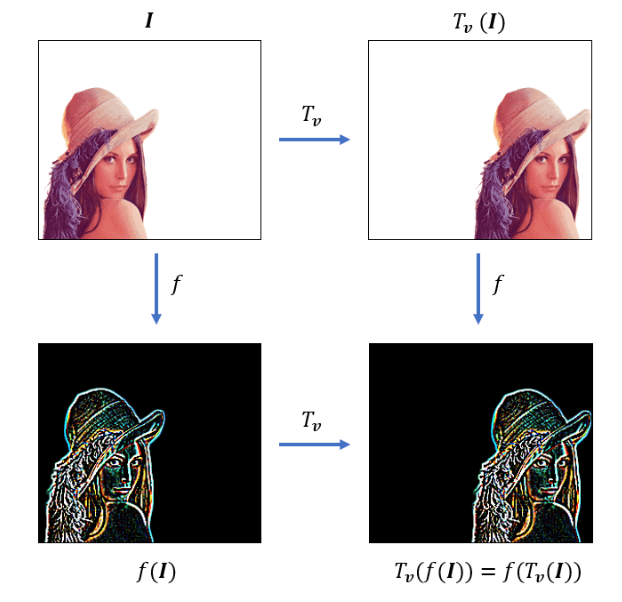
\includegraphics[width=0.5\textwidth]{../figures/equivariance.png}
    \end{center}
\end{frame}
%%%%%%%%%%%%%%%%%%%%%%%%%%%%%%%%%%%%%%%%%%%%%%%%%%%%%%%%%%%%%%%%%%%%%%%%%%%%%%



%%%%%%%%%%%%%%%%%%%%%%%%%%%%%%%%%%%%%%%%%%%%%%%%%%%%%%%%%%%%%%%%%%%%%%%%%%%%%%
\begin{frame}{Motivation}
    \begin{itemize}
        \setlength{\itemsep}{\fill}
        \item A cat is a cat no matter how you look at it.
    \end{itemize}

    \begin{center}
        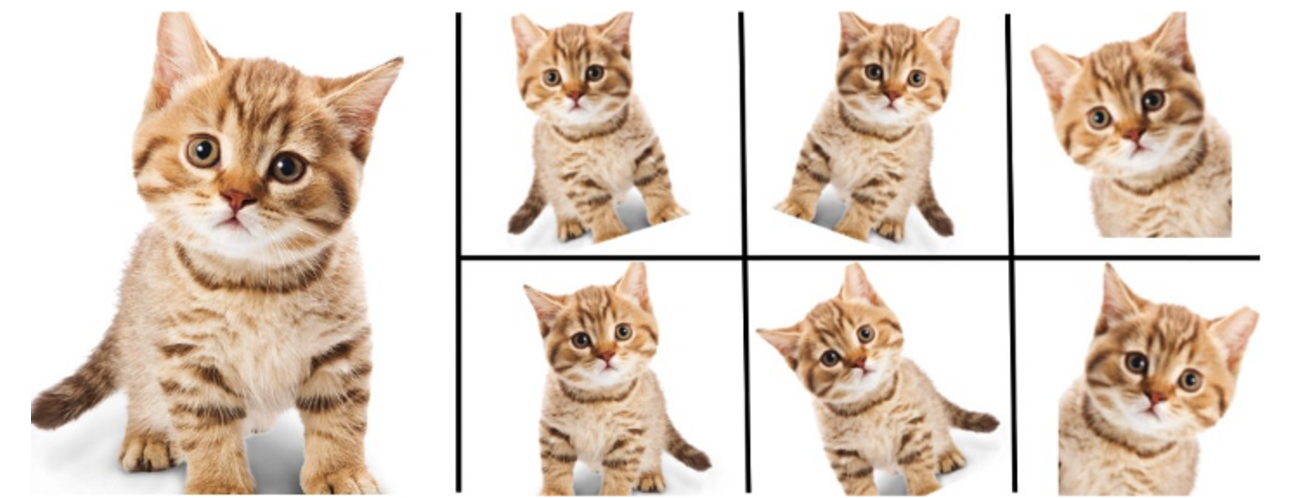
\includegraphics[width=0.8\textwidth]{../figures/cat.png}
    \end{center}

    \begin{itemize}
        \setlength{\itemsep}{\fill}
        %\pause
        \item It is acceptable to assume that being invariant to the rotation of the cat is a good property for a classification network.
    \end{itemize}
\end{frame}
%%%%%%%%%%%%%%%%%%%%%%%%%%%%%%%%%%%%%%%%%%%%%%%%%%%%%%%%%%%%%%%%%%%%%%%%%%%%%%



%%%%%%%%%%%%%%%%%%%%%%%%%%%%%%%%%%%%%%%%%%%%%%%%%%%%%%%%%%%%%%%%%%%%%%%%%%%%%%
\begin{frame}{Motivation}
    \begin{itemize}
        \setlength{\itemsep}{\fill}
        \item Our focus today is on sets and graph data.
        \end{itemize}
    \begin{center}
        \begin{minipage}[t]{0.69\textwidth}
            \centering
            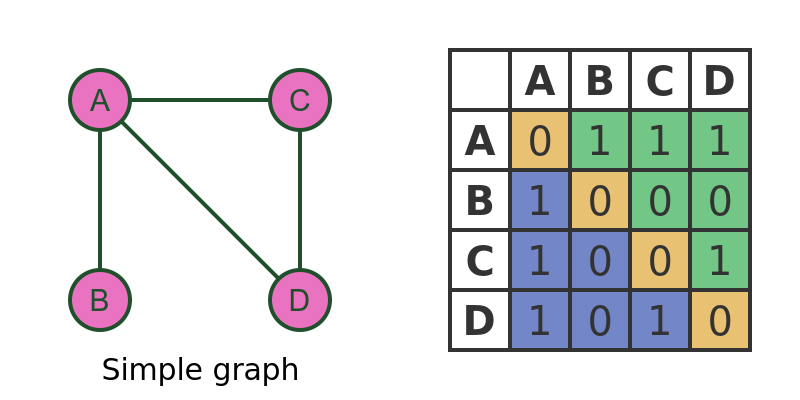
\includegraphics[width=\textwidth]{../figures/graph_adj.png}
        \end{minipage}
        \hfill
        \begin{minipage}[t]{0.3\textwidth}
            \centering
            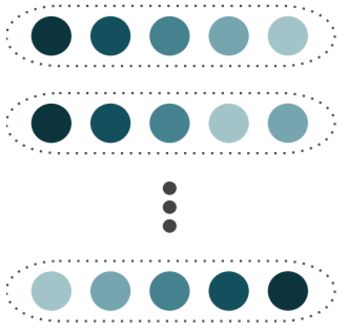
\includegraphics[width=\textwidth]{../figures/set.png}
        \end{minipage}
    \end{center}

\end{frame}
%%%%%%%%%%%%%%%%%%%%%%%%%%%%%%%%%%%%%%%%%%%%%%%%%%%%%%%%%%%%%%%%%%%%%%%%%%%%%%
\begin{frame}{Construction of an Equivariant Neural Network}
    When contructing an equivariant neural network, two things should always be considered:
    \begin{itemize} 
        \setlength{\itemsep}{\fill}
            %\pause
        \item The symmetries of the data:
        \begin{itemize}
            \item What inherent structure should our model be oblivious to?
        \end{itemize}
        \item The space of functions learnable by the network:\\ 
        \begin{itemize}
            \item Are we fully utilizing the space of functions that are equivariant to the symmetries of the data?
        \end{itemize}
    \end{itemize}
    
\end{frame}
%%%%%%%%%%%%%%%%%%%%%%%%%%%%%%%%%%%%%%%%%%%%%%%%%%%%%%%%%%%%%%%%%%%%%%%%%%%%%%

\section{Mathematical Background}

%%%%%%%%%%%%%%%%%%%%%%%%%%%%%%%%%%%%%%%%%%%%%%%%%%%%%%%%%%%%%%%%%%%%%%%%%%%%%%



%%%%%%%%%%%%%%%%%%%%%%%%%%%%%%%%%%%%%%%%%%%%%%%%%%%%%%%%%%%%%%%%%%%%%%%%%%%%%%
\begin{frame}{The Permutation Group $S_n$}

    \begin{itemize}
        \setlength{\itemsep}{\fill}
        \item The permutation group $S_n$ is the group of all permutations of $n$ elements.
        \item It has $n!$ elements, representing the $n!$ ways to order $n$ elements.
        \item Given a set $X = \{x_1, x_2, \ldots, x_n\}$, a permutation $\pi \in S_n$ is a bijection $\pi: X \rightarrow X$
        \item e.g. $x = (x_1, x_2, x_3)$, and $\pi = (1, 2, 3) \in S_3$ is the permutation that maps $1 \rightarrow 2$, $2 \rightarrow 3$ and $3 \rightarrow 1$.
        \item We denote the \textbf{action} of $\pi$ on $x$ as $\pi x = (x_3, x_1, x_2)$. 
    \end{itemize}

    
\end{frame}
%%%%%%%%%%%%%%%%%%%%%%%%%%%%%%%%%%%%%%%%%%%%%%%%%%%%%%%%%%%%%%%%%%%%%%%%%%%%%%



%%%%%%%%%%%%%%%%%%%%%%%%%%%%%%%%%%%%%%%%%%%%%%%%%%%%%%%%%%%%%%%%%%%%%%%%%%%%%%
\begin{frame}{Permutation Invariance}

    \begin{itemize}
        \setlength{\itemsep}{\fill}
        \item Let $H \leq S_n$ be a subgroup of the symmetric group.
        %\pause
        \item $f:\mathbb{R}^n \rightarrow \mathbb{R}$ is $H$-\textit{invariant} if $f(x) = f(\pi x)$ for all $\pi \in H$.
    \end{itemize}
    \begin{center}
        %\pause
        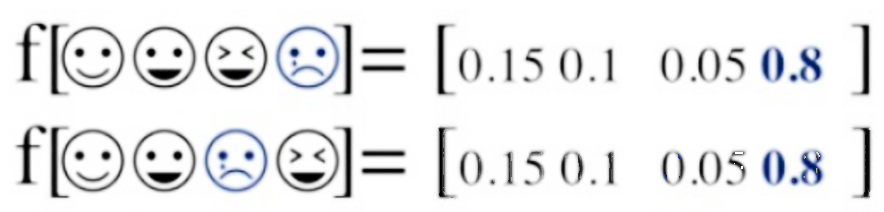
\includegraphics[width=0.65\textwidth]{../figures/perm_in.png}
    \end{center}
    
\end{frame}
%%%%%%%%%%%%%%%%%%%%%%%%%%%%%%%%%%%%%%%%%%%%%%%%%%%%%%%%%%%%%%%%%%%%%%%%%%%%%%



%%%%%%%%%%%%%%%%%%%%%%%%%%%%%%%%%%%%%%%%%%%%%%%%%%%%%%%%%%%%%%%%%%%%%%%%%%%%%%
\begin{frame}{Permutation Equivariance}

    \begin{itemize}
        \setlength{\itemsep}{\fill}
        \item Let $H \leq S_n$ be a subgroup of the symmetric group.
        %\pause
        \item $f:\mathbb{R}^n \rightarrow \mathbb{R}^n$ is \textit{permutation equivariant} if $\pi f(x) = f(\pi x)$ for all $\pi \in H$.
    \end{itemize}
    \begin{center}
        %\pause
        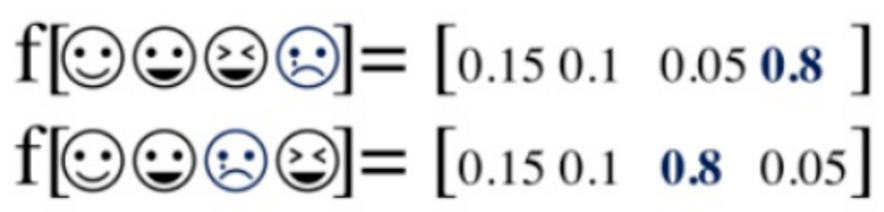
\includegraphics[width=0.65\textwidth]{../figures/perm_eq.png}
    \end{center}
    
\end{frame}
%%%%%%%%%%%%%%%%%%%%%%%%%%%%%%%%%%%%%%%%%%%%%%%%%%%%%%%%%%%%%%%%%%%%%%%%%%%%%%



%%%%%%%%%%%%%%%%%%%%%%%%%%%%%%%%%%%%%%%%%%%%%%%%%%%%%%%%%%%%%%%%%%%%%%%%%%%%%%
\begin{frame}{Permutation of a Set}

    \begin{itemize}
        \setlength{\itemsep}{\fill}
        \item Assume our set is $X = \{x_1, x_2, \ldots, x_n\}$.
        %\pause
        \item We can represent $X$ as a matrix $X \in \mathbb{R}^{n \times d}$.
        %\pause
        \item Any permutation $g \in S_n$ can be represented as a permutation matrix $\boldsymbol{P} \in \mathbb{R}^{n \times n}$,
        %\pause
        \item The action of $g$ on $X$ is then $\boldsymbol{P} X$.
        %\pause
        \item An invariant neural network is a function $f: \mathbb{R}^{n \times d} \rightarrow \mathbb{R}^{d`}$ such that $f(X) = f(\boldsymbol{P}X)$.
        %\pause
        \item An equivariant neural network is a function $f: \mathbb{R}^{n \times d} \rightarrow \mathbb{R}^{n \times d`}$ such that $\boldsymbol{P}f(X) = f(\boldsymbol{P}X)$.
    \end{itemize}
    
\end{frame}
%%%%%%%%%%%%%%%%%%%%%%%%%%%%%%%%%%%%%%%%%%%%%%%%%%%%%%%%%%%%%%%%%%%%%%%%%%%%%%


%%%%%%%%%%%%%%%%%%%%%%%%%%%%%%%%%%%%%%%%%%%%%%%%%%%%%%%%%%%%%%%%%%%%%%%%%%%%%%
\begin{frame}{Permutation of a Graph}

    \begin{itemize}
        \setlength{\itemsep}{\fill}
        \item Our data is now a graph adjacency matric $A \in \mathbb{R}^{n \times n}$. 
        %\pause
        \item A permutation matrix $\boldsymbol{P} \in \mathbb{R}^{n \times n}$ acts on the adjacency matrix $A$.
        %\pause
        \item The action of $\boldsymbol{P}$ on $A$ is:
        \[ \boldsymbol{P^T}A\boldsymbol{P} \]
    \end{itemize}
    
\end{frame}
%%%%%%%%%%%%%%%%%%%%%%%%%%%%%%%%%%%%%%%%%%%%%%%%%%%%%%%%%%%%%%%%%%%%%%%%%%%%%%
\begin{frame}{Permutation of a Graph}
    \begin{center}
        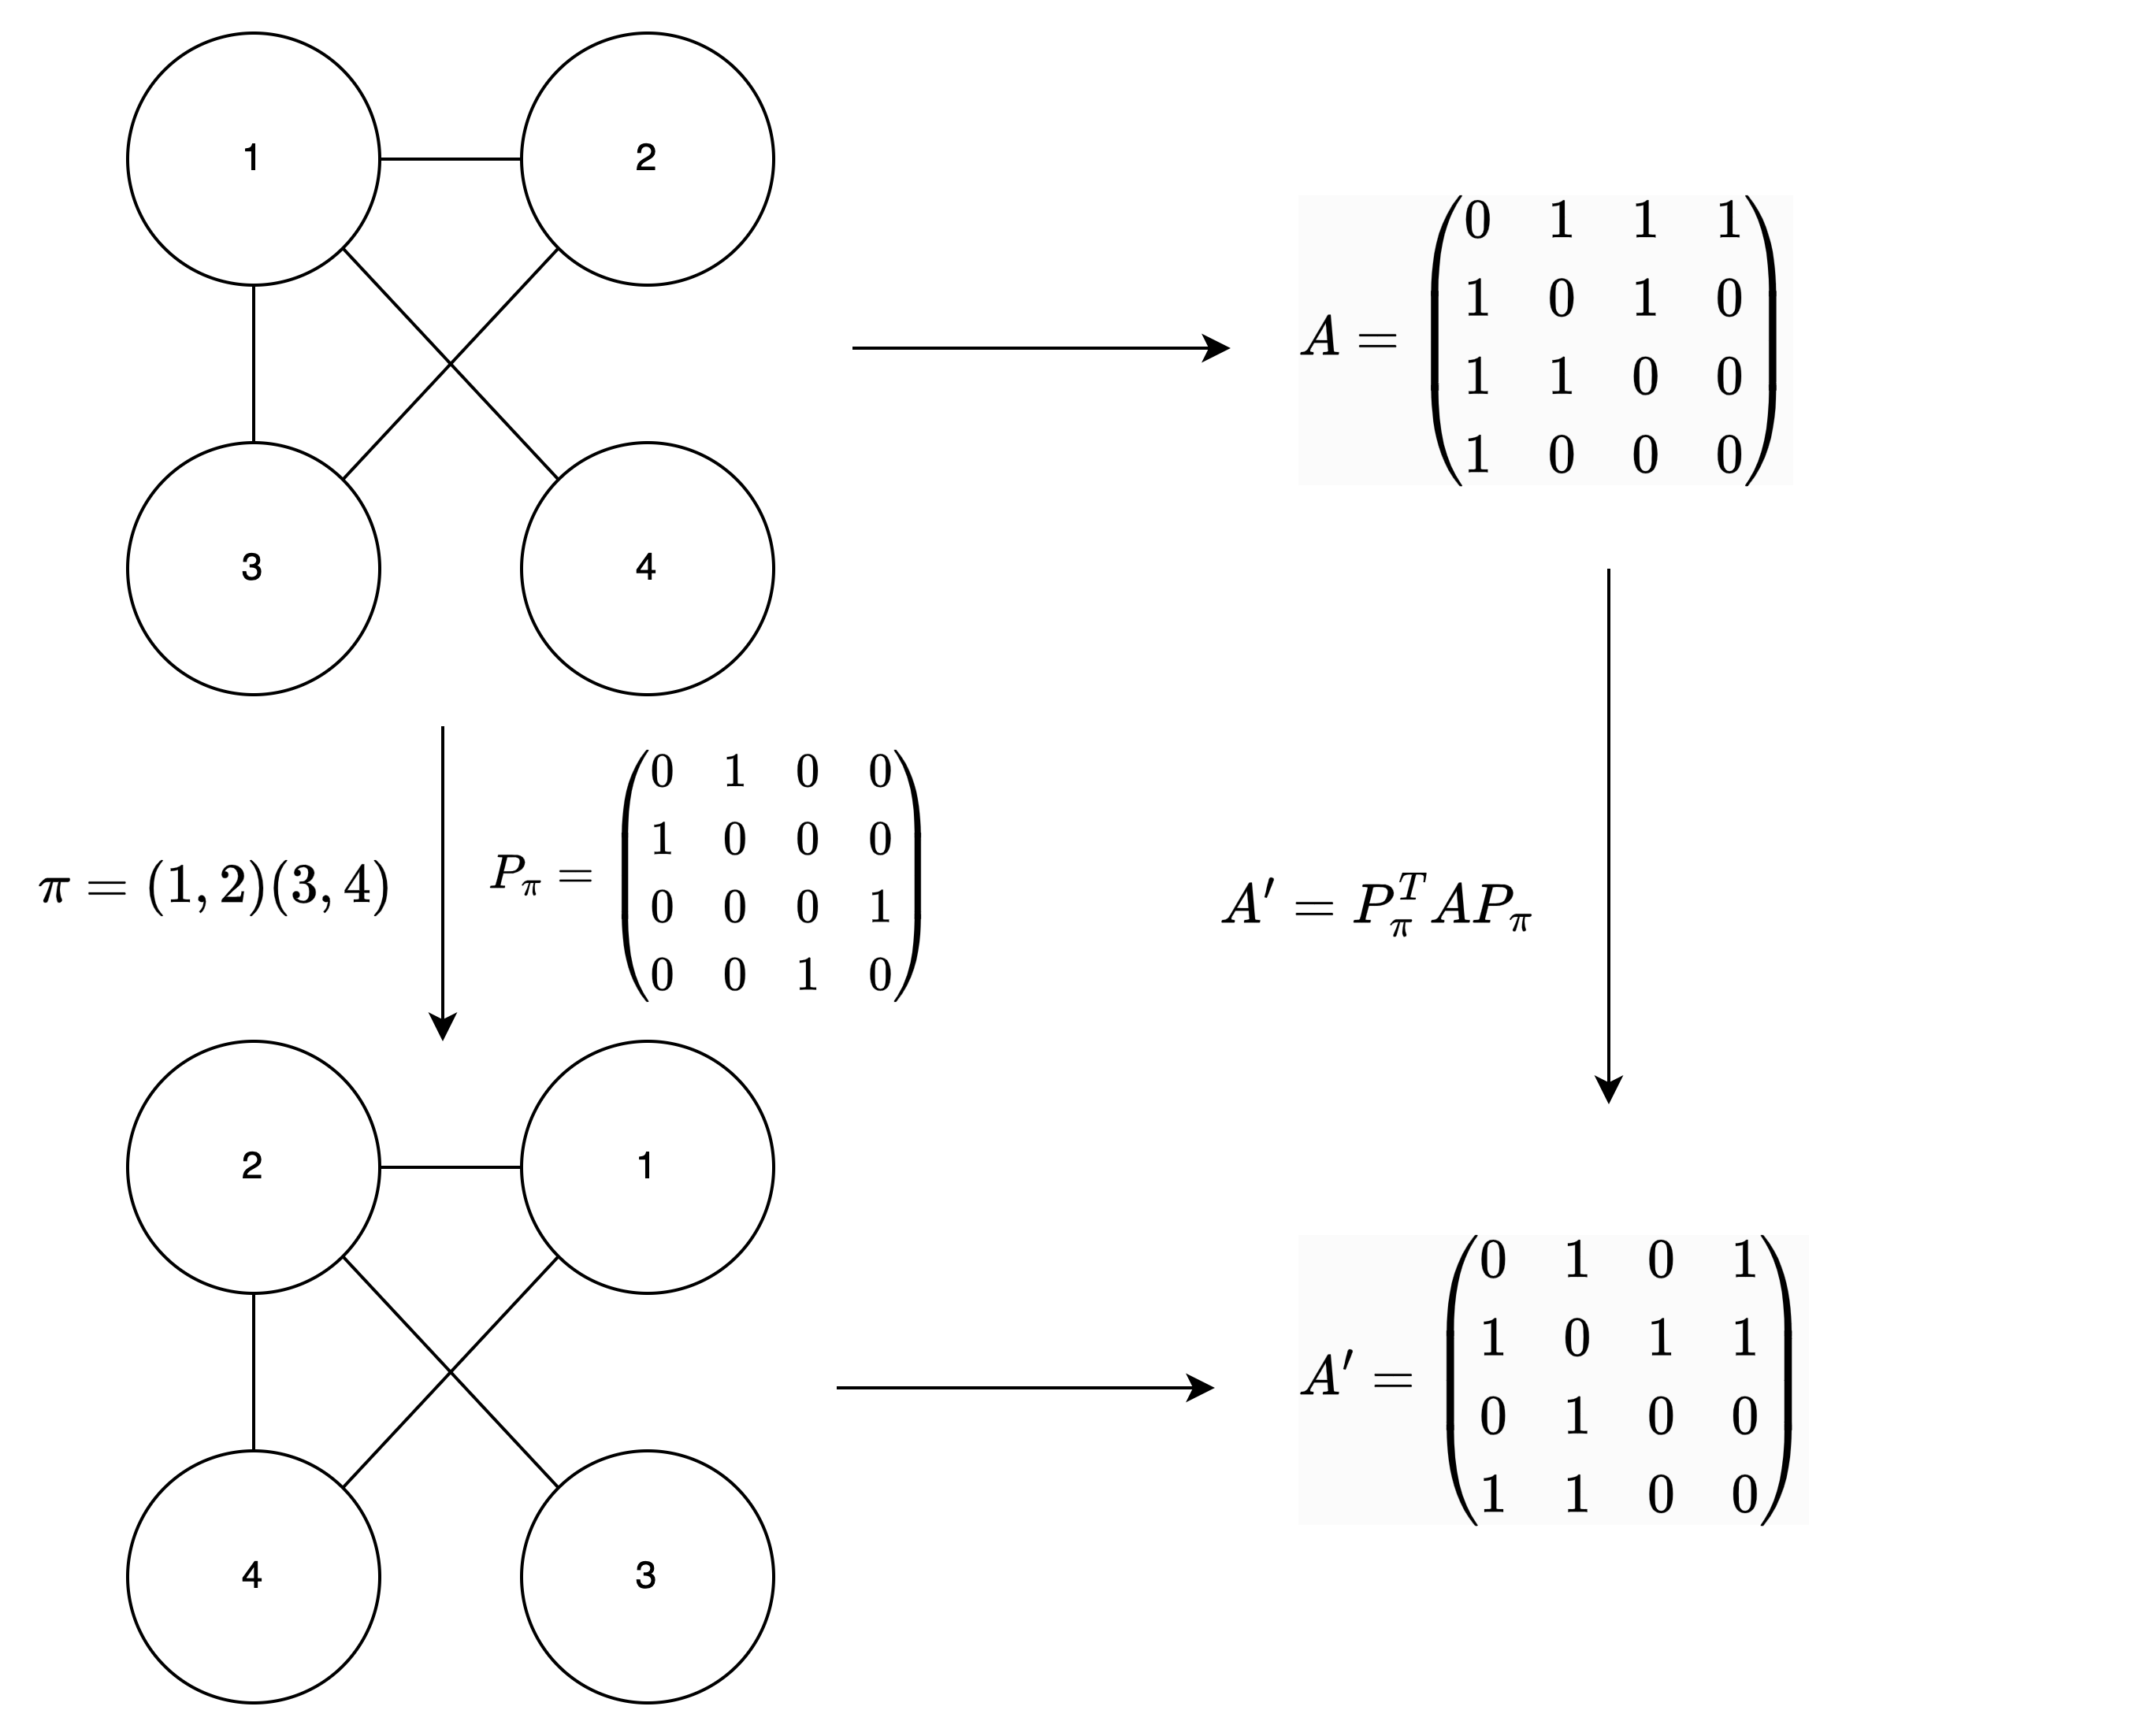
\includegraphics[width=0.8\textwidth]{../figures/node_permutation.png}
    \end{center}
\end{frame}
%%%%%%%%%%%%%%%%%%%%%%%%%%%%%%%%%%%%%%%%%%%%%%%%%%%%%%%%%%%%%%%%%%%%%%%%%%%%%%

\begin{frame}{Equivariant Network Construction}

    \begin{theorem}
        Let $L$ be a linear equivariant layer, and let $f$ be a neural network constructed be stacking $L$ and non-linearities $\sigma$. Then $f$ is permutation equivariant.
    \end{theorem}
    %\pause
    \begin{proof}
        Let $x$ be a set of $n$ elements, and let $g \in S_n$ be a permutation.
        %\pause
        \[ f(gx) = L(\sigma(L(\sigma(\ldots L(gx) \ldots)))) = L(\sigma(L( \ldots g\sigma(L(x)) \ldots))) = \ldots \]
        %\pause
        \[ g L(\sigma(L(\sigma(\ldots L(x) \ldots)))) = gf(x) \]
    \end{proof}
    
    
\end{frame}

%%%%%%%%%%%%%%%%%%%%%%%%%%%%%%%%%%%%%%%%%%%%%%%%%%%%%%%%%%%%%%%%%%%%%%%%%%%%%%
\begin{frame}{Invariant Network Construction}
    \begin{theorem}
        Let $f$ be an equvariant neural network and let $\phi$ be a permutation invariant function. Then $h = \phi(f(x))$ is a permutation invariant neural network.
    \end{theorem}
    %\pause
    \begin{proof}
        Let $x$ be a set of $n$ elements, and let $g \in S_n$ be a permutation.
        %\pause
        \[ h(gx) = \phi(f(gx)) = \phi(gf(x)) = \phi(f(x)) = h(x) \]
    \end{proof}
\end{frame}

%%%%%%%%%%%%%%%%%%%%%%%%%%%%%%%%%%%%%%%%%%%%%%%%%%%%%%%%%%%%%%%%%%%%%%%%%%%%%%

\section{Deep Sets}

%%%%%%%%%%%%%%%%%%%%%%%%%%%%%%%%%%%%%%%%%%%%%%%%%%%%%%%%%%%%%%%%%%%%%%%%%%%%%%
\begin{frame}{Deep Sets}

    \begin{itemize}
        \setlength{\itemsep}{\fill}
        \item A seminal work in the field of equivariant neural networks. 
        %\pause
        \item Recall the two properties we mentioned earlier (symmetries of the data and the space of functions learnable by the network).
        %\pause
        \item \emph{DeepSets} is an architecture that is equivariant to set permutations and is maximally expressive in the space of permutation equivariant functions.
        %\pause
        \item We are going to see the construction and prove it satisfies equivariance and expressiveness.
    \end{itemize}
    
\end{frame}
%%%%%%%%%%%%%%%%%%%%%%%%%%%%%%%%%%%%%%%%%%%%%%%%%%%%%%%%%%%%%%%%%%%%%%%%%%%%%%
\begin{frame}{\emph{DeepSets} Layer}

    \begin{itemize}
        \setlength{\itemsep}{\fill}
        \item We saw a general structure of an invariant and equivariant network.
        \item To fill in the details, we need to define the equivariant layer $L$ and the invariant function $\phi$.
    \end{itemize}

    %\pause
    \begin{definition}
        Consider a set $x = \{x_1, x_2, \ldots, x_n\}$, where $x_i \in \mathbb{R}$. Define its representation $\mathbf{x} = (x_1, \dots, x_n) \in \mathbb{R}^n$.\\
        A \emph{DeepSets} layer is defined as 
        \[L(x) = \lambda\mathrm{I}\mathbf{x} + \mathbf{x}\mathbf{1}\].
    \end{definition}
    
\end{frame}
%%%%%%%%%%%%%%%%%%%%%%%%%%%%%%%%%%%%%%%%%%%%%%%%%%%%%%%%%%%%%%%%%%%%%%%%%%%%%%
\begin{frame}{\emph{DeepSets} Layer}

    \begin{definition}
        Consider a set $x = \{x_1, x_2, \ldots, x_n\}$, where $x_i \in \mathbb{R}$.\\
        A \emph{DeepSets} layer is defined as 
        \[L(x) = \lambda\mathrm{I}\mathbf{x} + \mathbf{x}\mathbf{1}\].
    \end{definition}

    %\pause
    \begin{theorem}
        A \emph{DeepSets} layer is permutation equivariant.
    \end{theorem}

    %\pause
    \begin{proof}
        Let $x$ be a set of $n$ elements, and let $g \in S_n$ be a permutation.
        %\pause
        \[ L(gx) = \lambda\mathrm{I}(gx) + (gx)\mathbf{1} = g(\lambda\mathrm{I}x) + x\mathbf{1} = gL(x)\]
    \end{proof}
\end{frame}
%%%%%%%%%%%%%%%%%%%%%%%%%%%%%%%%%%%%%%%%%%%%%%%%%%%%%%%%%%%%%%%%%%%%%%%%%%%%%%
\begin{frame}{\emph{DeepSets} Layer}
    %\pause
    \begin{theorem}
        Any linear equivariant layer is of the shape \(L(x) = \lambda\mathrm{I}\mathbf{x} + \mathbf{x}\mathbf{1}\).
    \end{theorem}

    %\pause
    \renewcommand{\qedsymbol}{}
    \begin{proof}[Proof (through example)]
        Let $\mathbf{x}=\{x_1,x_2,x_3\}$ be a set, $W \in \mathbb{R}^{3 \times 3}$, and $L(x) = W\mathbf{x}$ such that $L$ is equivariant, W = $\begin{pmatrix}
            a & b & c\\
            d & e & f\\
            g & h & i
        \end{pmatrix}$.\\
        %\pause
        Consider permutation $g=(2,3) \in S_3$. Note that $g\left(W\begin{pmatrix}
            x_1\\
            x_2\\
            x_3
        \end{pmatrix}\right)_1=(Wx)_1 = (Wgx)_1 = \left(W\begin{pmatrix}
            x_1\\
            x_3\\
            x_2
        \end{pmatrix}\right)_1$\\
    \end{proof}
    \renewcommand{\qedsymbol}{\ensuremath{\square}} 
\end{frame}
%%%%%%%%%%%%%%%%%%%%%%%%%%%%%%%%%%%%%%%%%%%%%%%%%%%%%%%%%%%%%%%%%%%%%%%%%%%%%%
\begin{frame}{\emph{DeepSets} Layer}
    \renewcommand{\qedsymbol}{} 
    \begin{proof}[Proof (through example) - continued]
        {\footnotesize
        The previous equation can be written as:
        \[ax_1 + bx_2 + cx_3 = ax_1 + bx_3 + cx_2\]
        This should hold for any choice of $\mathbf{x}$ $\Rightarrow b = c$, $d=f, g=h$. \\
        %\pause
        For the permutation $\sigma = (1,3,2)$:  
        
        \[W(\sigma x) = W \begin{pmatrix}
            x_2 \\
            x_3 \\
            x_1
        \end{pmatrix} = 
        \begin{pmatrix}
            ax_2 + bx_3 + bx_1 \\
            dx_2 + ex_3 + dx_1 \\
            fx_2 + fx_3 + ix_1
        \end{pmatrix}\]
        \[
        \sigma W \begin{pmatrix}
            x_1 \\
            x_2 \\
            x_3
        \end{pmatrix} = (1,3, 2) \begin{pmatrix}
            ax_1 + bx_2 + bx_3 \\
            dx_1 + ex_2 + dx_3 \\
            fx_1 + fx_2 + ix_3
        \end{pmatrix} = \begin{pmatrix}
            dx_1 + ex_2 + dx_3 \\
            fx_1 + fx_2 + ix_3 \\
            ax_1 + bx_2 + bx_3
        \end{pmatrix} \stackrel{!}{=} \] \\
        \[ = W \begin{pmatrix}
            x_2 \\
            x_3 \\
            x_1
        \end{pmatrix}
        \]
        }
    \end{proof}
    \renewcommand{\qedsymbol}{\ensuremath{\square}} 
\end{frame}
%%%%%%%%%%%%%%%%%%%%%%%%%%%%%%%%%%%%%%%%%%%%%%%%%%%%%%%%%%%%%%%%%%%%%%%%%%%%%%

\begin{frame}{\emph{DeepSets} Layer}
    \begin{proof}[Proof (through example) - continued]
        We can use the same logic to show that $a = e = i$, $b = c = d = f = g = h$.\\
        We get that all values in the diagonal must be equal and all values in the off-diagonal must be equal, and $W$ must have the form:
        \[W = \begin{pmatrix}
            a & b & b\\
            b & a & b\\
            b & b & a
        \end{pmatrix}\].
    \end{proof}
\end{frame}
%%%%%%%%%%%%%%%%%%%%%%%%%%%%%%%%%%%%%%%%%%%%%%%%%%%%%%%%%%%%%%%%%%%%%%%%%%%%%%
\begin{frame}{\emph{DeepSets} Network}
    \begin{itemize}
        \setlength{\itemsep}{\fill}
        \item We have an initial layer $L$, which we proved is equivariant.
        %\pause
        \item A deep sets invariant network is now constructed as:\\
        \[f(x) = \phi(L\sigma(L\sigma(\ldots L\sigma(L(x)) \ldots))) \quad \text{where} \quad \phi(x) = \sum_{i=1}^{n}x_i \]
        %\pause
        \item It is easy to see that $\phi$ is permutation invariant, and thus $f$ is permutation invariant.
        \item For a classification network, take some classification module $\rho$ (e.g. an MLP), and define the final network as:
        \[ h(x) = \rho(f(x)) \]  
    \end{itemize}
\end{frame}
%%%%%%%%%%%%%%%%%%%%%%%%%%%%%%%%%%%%%%%%%%%%%%%%%%%%%%%%%%%%%%%%%%%%%%%%%%%%%%
\begin{frame}{\emph{DeepSets} Network}
    \begin{itemize}
        \setlength{\itemsep}{\fill}
        \item Notice that the network is only defined for sets with elements in $\mathbb{R}$.
        \item We can extend this to a set $X = \{x_1, x_2, \dots x_n\} \subset \mathbb{R}^d$ with representation $\textbf{X}\in\mathbb{R}^{n \times d}$ by defining $L$ as:
        \[L(x) = \mathbf{X}W_1 + \mathbf{1}\mathbf{1}^T\mathbf{X}W_2\]
        \item This keeps the general structure of the layer: a linear transformation of the distinct elements of the set summed with the mean of the set.  
    \end{itemize}
\end{frame}
%%%%%%%%%%%%%%%%%%%%%%%%%%%%%%%%%%%%%%%%%%%%%%%%%%%%%%%%%%%%%%%%%%%%%%%%%%%%%%
\begin{frame}{\emph{DeepSets} Expressivity}
    \begin{itemize}
        \setlength{\itemsep}{\fill}
        \item We have shown that the \emph{DeepSets} network is permutation invariant.
        %\pause
        \item We now want to show that it is maximally expressive in the space of permutation invariant functions.
        %\pause
        \item We show outline for the proof, showing \emph{DeepSets} can separate any two sets that are not equal.

    \end{itemize}
    %\pause
    \begin{theorem}
        Let $x,y \in \mathbb{R}^{n \times d} \quad$ s.t $\quad x \neq gy \quad \forall g \in S_n$. Then there exists a \emph{DeepSets} network that separates $x$ and $y$, namely $F(x ; \theta) \neq F(y ; \theta)$. 
    \end{theorem}
    
    

\end{frame}
%%%%%%%%%%%%%%%%%%%%%%%%%%%%%%%%%%%%%%%%%%%%%%%%%%%%%%%%%%%%%%%%%%%%%%%%%%%%%%
\begin{frame}{\emph{DeepSets} Expressivity}
    Proof outline:
    \begin{enumerate}
        \setlength{\itemsep}{\fill}
        %\pause
        \item Consider distinct rows of $x, y$.
        %\pause
        \item Construct input output pairs using standard basis elements (one hot encodings of the elements in the set).
        \item In each layer $L(x) = \mathbf{X}W_1 + \mathbf{1}\mathbf{1}^T\mathbf{X}W_2$, set $W_2 = 0$, collapsing our network to a standard MLP.
        %\pause
        \item According to a result of the universal approximation theorem, we can learn a one to one mapping between the input and output pairs.
        %\pause
        \item Output for each set the sum of the output pairs.
        %\pause
        \item For each set, we computed the  hitogram of its elements, which is a unique representation of the set.
    \end{enumerate}


\end{frame}
%%%%%%%%%%%%%%%%%%%%%%%%%%%%%%%%%%%%%%%%%%%%%%%%%%%%%%%%%%%%%%%%%%%%%%%%%%%%%%

\section{Invariant and Equivariant Graph Networks}

%%%%%%%%%%%%%%%%%%%%%%%%%%%%%%%%%%%%%%%%%%%%%%%%%%%%%%%%%%%%%%%%%%%%%%%%%%%%%%
\begin{frame}{Invariant and Equivariant Graph Networks}
    \begin{itemize}
        \setlength{\itemsep}{\fill}
        \item We saw a simple, maximally expressive equivariant network for sets.
        %\pause
        \item We now want to extend this to graphs.
    \end{itemize}
\end{frame}
%%%%%%%%%%%%%%%%%%%%%%%%%%%%%%%%%%%%%%%%%%%%%%%%%%%%%%%%%%%%%%%%%%%%%%%%%%%%%%
\begin{frame}{Invariant and Equivariant Graph Networks}
    \begin{itemize}
        \setlength{\itemsep}{\fill}
        \item Recall the action of the permutation matrix $\boldsymbol{P}$ on the adjacency matrix $A$ is:
        \[\boldsymbol{P^T}A\boldsymbol{P}\]
        %\pause
        \item Let's use this to define a linear invariant layer $L \in \text{Hom}(\mathbb{R}^{n\times n}, \mathbb{R})$. We want to satisfy the following:
        \[ L(\boldsymbol{P^T}A\boldsymbol{P}) = L(A) \]
        \item It's hard from this to understand the conditions on $L$. 
        \pause
        \item We define an equivalent condition by column stacking the adjacency matrix to get a vector, and then looking at $L$'s matrix representation: $\mathbf{L} \in \mathbb{R}^{1 \times n^2}$.
        \[ \mathbf{L}\text{vec}(\boldsymbol{P}^T A\boldsymbol{P}) = \mathbf{L}\text{vec}(A) \]
        %\pause
    \end{itemize}
\end{frame}
%%%%%%%%%%%%%%%%%%%%%%%%%%%%%%%%%%%%%%%%%%%%%%%%%%%%%%%%%%%%%%%%%%%%%%%%%%%%%%
\begin{frame}{Invariant and Equivariant Graph Networks}
    \begin{itemize}
        \setlength{\itemsep}{\fill}
        \item What if our adjacency matrix is actually a tensor $\mathbf{A} \in \mathbb{R}^{n^k}$?
        \item Instead of looking at relationships between pairs of nodes, we now look at relationships between $k$-tuples of nodes.
        \item We want to extend the previous condition \(\mathbf{L}\text{vec}(\boldsymbol{P} \circ \mathbf{A}) = \mathbf{L}\text{vec}(A)\) to hold for any $A$.
        \item Note that the action of $\boldsymbol{P}$ on $\mathbf{A}$ is not necessarily $\boldsymbol{P}^T \mathbf{A} \boldsymbol{P}$ as this may not be defined over $k$-order tensors. 
    \end{itemize}
\end{frame}
%%%%%%%%%%%%%%%%%%%%%%%%%%%%%%%%%%%%%%%%%%%%%%%%%%%%%%%%%%%%%%%%%%%%%%%%%%%%%%
\begin{frame}{Invariant and Equivariant Graph Networks}
    \begin{itemize}
        \setlength{\itemsep}{\fill}
        \item We now introduce a crucial property of the Kronecker product:
        \[ \text{vec}(XAY)= Y^T\otimes X\text{vec}(A)\]
        %\pause
        \item Using this, the previous condition can be written as:
        \[ L(P^T\otimes P^T)\text{vec}(A) = L\text{vec}(A) \]
        %\pause
        \item For this condition to hold for all $A$, we need $L$ to satisfy:
        \[ L(P^T\otimes P^T) = L \]
        %\pause
        \item transposing the equation, and with severe abuse of notation $(L^T = \text{vec(L)})$, we finally get:
        \[ (P\otimes P)\text{vec}(L) = \text{vec}(L) \]
    \end{itemize}
\end{frame}
%%%%%%%%%%%%%%%%%%%%%%%%%%%%%%%%%%%%%%%%%%%%%%%%%%%%%%%%%%%%%%%%%%%%%%%%%%%%%%
\begin{frame}{Invariant and Equivariant Graph Networks}
    \begin{itemize}
        \setlength{\itemsep}{\fill}
        \item After some work and moderate logic jumps, we got a condition for a permutation invariant linear layer $L$.
        %\pause
        \item Developing the condition for an equivariant layer $L \in \mathbb{R}^{n^2 \times n^2}$ is very similar:
        %\pause
        \[ L\text{vec}(\boldsymbol{P}^T A\boldsymbol{P}) =\boldsymbol{P}^T L\text{vec}(A) \boldsymbol{P}\]
        %\pause
        \item Using the Kronecker product property, we get:
        \[ L(P^T\otimes P^T)\text{vec}(A) = (P^T\otimes P^T)L\text{vec}(A) \]
        %\pause
        \item This should hold for every $A$, so we get:
        \[ L(P^T\otimes P^T) = (P^T\otimes P^T)L \]
    \end{itemize}
\end{frame}
%%%%%%%%%%%%%%%%%%%%%%%%%%%%%%%%%%%%%%%%%%%%%%%%%%%%%%%%%%%%%%%%%%%%%%%%%%%%%%
\begin{frame}{Invariant and Equivariant Graph Networks}
    \begin{itemize}
        \setlength{\itemsep}{\fill}
        \item $(P^T\otimes P^T)$ is an $n^2 \times n^2$ permutation matrix, and its inverse is $(P\otimes P)$.
        %\pause
        \[ (P\otimes P)L(P^T\otimes P^T) = L \]
        \item Once again using the Kronecker product property, we get:
        \[ \text{vec}(L) = \text{vec}(P\otimes P)L(P^T\otimes P^T) = (P\otimes P) \otimes (P \otimes P) \text{vec}(L) \]
        \[ = (P \otimes P \otimes P \otimes P) \text{vec}(L) \]
        %\pause
        \item The previous conditions are developed for a matrix $A \in \mathbb{R}^{n^2}$ expressing the relations between pairs of nodes.
        \item We can extend this to a matrix $A \in \mathbb{R}^{n^k}$ expressing the relations between every $k$ tuple of nodes.
        \item for invariant layers $L \in \mathbb{R}^{1 \times n^k}$:
        \[ P^{\otimes k}\text{vec}(L) = \text{vec}(L) \]
        \item for equivariant layers $L \in \mathbb{R}^{n^k \times n^k}$:
        \[ P^{\otimes 2k}L = \text{vec}(L) \]
    \end{itemize}
\end{frame}
%%%%%%%%%%%%%%%%%%%%%%%%%%%%%%%%%%%%%%%%%%%%%%%%%%%%%%%%%%%%%%%%%%%%%%%%%%%%%%
\begin{frame}{Invariant and Equivariant Graph Networks}
    \begin{itemize}
        \setlength{\itemsep}{\fill}
        \item We developed conditions for a permutation invariant and equivariant linear layer $L$. Call these the Fixed Point Equations.
        %\pause
        \item Unfortunately, compared to the simple structure of the \emph{DeepSets} layer, these equations are less interpretable. Let's try and make some sense of them.
        %\pause
        \item The condition we got is one that determines the values of the entries of $L$. We want to understand what entries of $L$ should be equal.
        %\pause
        \item For an invariant layer $L \in \mathbb{R}^{1 \times n^k}$, $L_{i_1,i_2,\ldots,i_k}$ is the weight which multiplies entry $A_{i_1,i_2,\ldots,i_k}$.
    \end{itemize}
\end{frame}
%%%%%%%%%%%%%%%%%%%%%%%%%%%%%%%%%%%%%%%%%%%%%%%%%%%%%%%%%%%%%%%%%%%%%%%%%%%%%%
\begin{frame}{Invariant and Equivariant Graph Networks}
    \begin{itemize}
        \setlength{\itemsep}{\fill}
        \item The Fixed Point Equation for an invariant layer is:
        \[ P^{\otimes k}\text{vec}(L) = \text{vec}(L) \]
        %\pause
        \item The k-th permutation matrix permutes the k-th dimension of the input. 
        \[ P^{\otimes k}\text{vec}(L)_{i_1, \ldots i_k} = \text{vec}(L)_{\sigma(i)_1, \ldots \sigma(i)_k} \]
        %\pause
        \item This partitions the entries of $L$ into equivalence classes, where all entries in the same class are equal.
        %\pause
        \item For $k=2$ we get 2 equivalence classes:
        \[ L_{i,j} \quad \text{where} \quad i \neq j \quad \text{and} \quad L_{i,i} \]
    \end{itemize}
\end{frame}
%%%%%%%%%%%%%%%%%%%%%%%%%%%%%%%%%%%%%%%%%%%%%%%%%%%%%%%%%%%%%%%%%%%%%%%%%%%%%%
\begin{frame}{Invariant and Equivariant Graph Networks}
    \begin{itemize}
        \setlength{\itemsep}{\fill}
        \item For an equivariant layer $L \in \mathbb{R}^{1 \times n^k}$, $L_{i_1,i_2,\ldots,i_k, j_1, j_2,\ldots,j_k}$ is the weight which multiplies entry $A_{i_1,i_2,\ldots,i_k}$ 
        and sends it to entry ${j_1,j_2,\ldots,j_k}$ of the output.
        %\pause
        \item The Fixed Point Equation for an equivariant layer is:
        \[ P^{\otimes 2k}\text{vec}(L) = \text{vec}(L) \]
        %\pause
        \item The k-th permutation matrix permutes the k-th dimension of the input. 
        \[ P^{\otimes 2k}\text{vec}(L)_{i_1,i_2,\ldots,i_k, j_1, j_2,\ldots,j_k} = \text{vec}(L)_{\sigma(i)_1, \ldots \sigma(i)_k, \sigma(j)_1, \ldots \sigma(j)_k} \]
        %\pause
        \item Once again, this partitions the entries of $L$ into equivalence classes.
        %\pause
        \item For $k=2$ we get 15 equivalence classes:
        \[ \{\{1\} \{2\} \{3\} \{4\}\}, \{\{1, 2\} \{3\} \{4\}\}, \{\{1\} \{2, 3\} \{4\}\} \ldots \{\{1, 2, 3, 4\}\}\]
        %\pause
        In general, the number of equivalence classes is $Bell(2k)$ for an (equivariant) invariant layer of order $k$
    \end{itemize}
\end{frame}
%%%%%%%%%%%%%%%%%%%%%%%%%%%%%%%%%%%%%%%%%%%%%%%%%%%%%%%%%%%%%%%%%%%%%%%%%%%%%%
\begin{frame}{Invariant and Equivariant Graph Networks}
    \begin{itemize}
        \setlength{\itemsep}{\fill}
        \item Did you notice somthing similar to the \emph{DeepSets} layer?
        %\pause
        \item The construction of the \emph{DeepSets} layer is identicle to the construction of an equivariant layer of order 1.
        %\pause
        \item We managed to generalize the equivariant layer to higher orders of node connectivity.
        %\pause
        \item We also managed to generalize the invariant layer to higher orders of node connectivity.
    \end{itemize}
\end{frame}
%%%%%%%%%%%%%%%%%%%%%%%%%%%%%%%%%%%%%%%%%%%%%%%%%%%%%%%%%%%%%%%%%%%%%%%%%%%%%%
\begin{frame}{Invariant and Equivariant Graph Networks}
    \begin{center}
        \begin{minipage}[t]{0.45\textwidth}
            \raggedright % Ensures the content aligns to the left
            \vspace{0pt} % Forces top alignment
            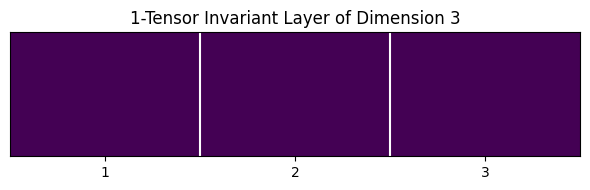
\includegraphics[width=\textwidth]{../figures/1-tensor-inv.png}
        \end{minipage}
        \hfill
        \begin{minipage}[t]{0.45\textwidth}
            \raggedright % Ensures the content aligns to the left
            \vspace{0pt} % Forces top alignment
            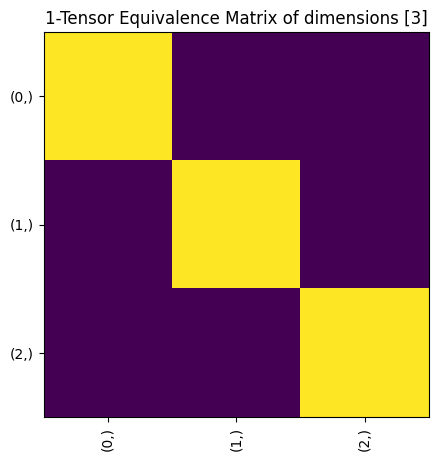
\includegraphics[width=\textwidth]{../figures/1-tensor-eq.png}
        \end{minipage}
    \end{center}
\end{frame}
%%%%%%%%%%%%%%%%%%%%%%%%%%%%%%%%%%%%%%%%%%%%%%%%%%%%%%%%%%%%%%%%%%%%%%%%%%%%%%
\begin{frame}{Invariant and Equivariant Graph Networks}
    \begin{center}
        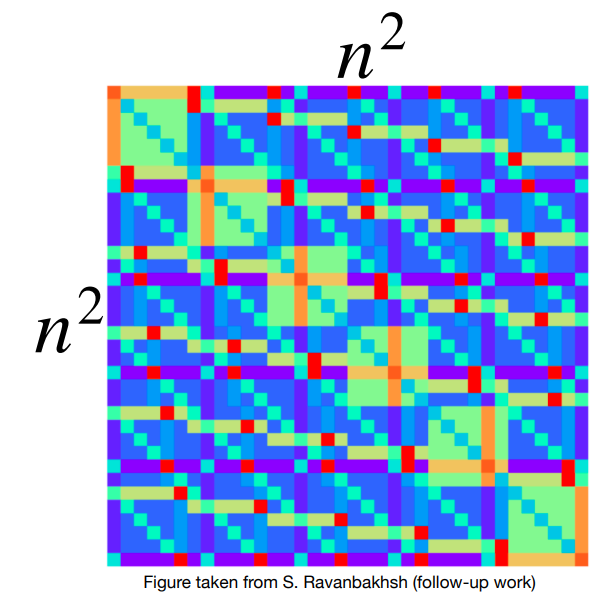
\includegraphics[width=0.65\textwidth]{../figures/2-tensor-eq.png}
    \end{center}
\end{frame}
%%%%%%%%%%%%%%%%%%%%%%%%%%%%%%%%%%%%%%%%%%%%%%%%%%%%%%%%%%%%%%%%%%%%%%%%%%%%%%
\begin{frame}{Invariant and Equivariant Graph Networks}
    \begin{itemize}
        \setlength{\itemsep}{\fill}
        \item Let's extend the construction of the equivariant layer even further, changing between the connectivity order, adding node features, and a bias term.
        %\pause
        \item We skip a few steps, but it makes sense that the bias term should satisfy the same fixed point equation as the linear term.
        \[ \mathbf{P}^{T \otimes k} \text{vec}(\mathbf{C}) = \text{vec}(\mathbf{C}) \]
        The main idea is that every pair of k-hyperedges which permute under some permutation should have the same bias term.
    \end{itemize}
\end{frame}
%%%%%%%%%%%%%%%%%%%%%%%%%%%%%%%%%%%%%%%%%%%%%%%%%%%%%%%%%%%%%%%%%%%%%%%%%%%%%%
\begin{frame}{Invariant and Equivariant Graph Networks}
    \begin{itemize}
        \setlength{\itemsep}{\fill}
        \item We can also consider node features.
        %\pause
        \item The input to the layer now includes a set of $n$ $d$-dimensional vectors.
        %\pause
        \item This is exactly the input to the \emph{DeepSets} layer, we already know how to construct an equivariant layer for this input.
        %\pause
        \item The input to our layer is now the k-connectivity of each node, concatenated with it's feature:
        \[ A \in \mathbb{R}^{n^k \times d} \]
        %\pause
        \item The new general formulation, changing both the connectivity order and the feature dimensionality, is:
        \[ L: \mathbb{R}^{n^k \times d} \rightarrow \mathbb{R}^{n^{k'} \times d'} \]
    \end{itemize}
\end{frame}
%%%%%%%%%%%%%%%%%%%%%%%%%%%%%%%%%%%%%%%%%%%%%%%%%%%%%%%%%%%%%%%%%%%%%%%%%%%%%%
\begin{frame}{Invariant and Equivariant Graph Networks}
    \begin{itemize}
        \setlength{\itemsep}{\fill}
        \item We intoduce some new notation, please bare with us as we will use some Nifnufey Yadaim.
        %\pause
        \item We saw certain entries of the layer matrix $L$ are equal.
        In \emph{DeepSets} our connectivity is of order 1, so we got 2 equivalence classes.
        In the standard graph case, our connectivity is of order 2, so we got 15 equivalence classes.
        \item These equivalence classes are completely disjoint, meaning every entry in the linear layer belongs to exactly one equivalence class.
    \end{itemize}
\end{frame}
%%%%%%%%%%%%%%%%%%%%%%%%%%%%%%%%%%%%%%%%%%%%%%%%%%%%%%%%%%%%%%%%%%%%%%%%%%%%%%
\begin{frame}{Invariant and Equivariant Graph Networks}
    \begin{itemize}
        \setlength{\itemsep}{\fill}
        \item Let $\mu$ be some equivalence class of indices. We denote by $\mathbf{M}^\mathbf{\mu}$ the binary tensor which is 1 at the indices in $\mathbf{\mu}$ and 0 elsewhere.
        %\pause
        \item Denote by $\mathbf{B}^\mathbf{\mu}, \mathbf{C}^\mathbf{\mu}$ the linear layer and bias term of the layer, respectively. 
        %\pause
        \item For an invariant layer $L: \mathbb{R}^{n^k \times d} \rightarrow \mathbb{R}^{n^1 \times d'}$, this defines a set of $dd'Bell(k) + d'$ binary tensors.
        %\pause
        \item For an equivariant layer $L: \mathbb{R}^{n^k \times d} \rightarrow \mathbb{R}^{n^{k'} \times d'}$, this defines a set of $dd'Bell(k+k') + d'Bell(k')$ binary tensors.
    \end{itemize}
\end{frame}
%%%%%%%%%%%%%%%%%%%%%%%%%%%%%%%%%%%%%%%%%%%%%%%%%%%%%%%%%%%%%%%%%%%%%%%%%%%%%%
\begin{frame}{Invariant and Equivariant Graph Networks}
    The full charactarization of the space of invariant and equivariant layers is:
    \begin{center}
        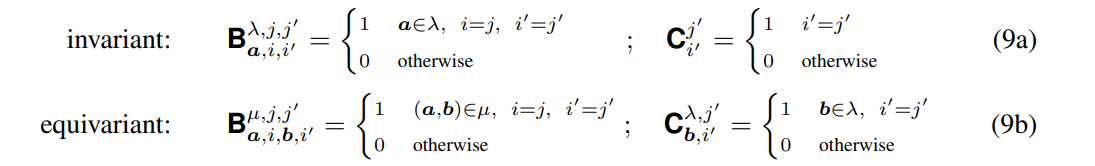
\includegraphics[width=0.9\textwidth]{../figures/layer_gener.png}
    \end{center}
    \begin{center}
        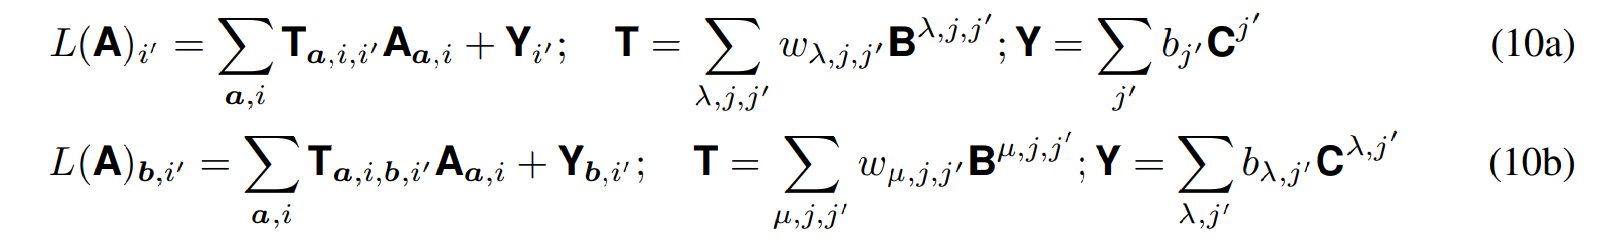
\includegraphics[width=0.9\textwidth]{../figures/full_formulation.png}
    \end{center}
\end{frame}
%%%%%%%%%%%%%%%%%%%%%%%%%%%%%%%%%%%%%%%%%%%%%%%%%%%%%%%%%%%%%%%%%%%%%%%%%%%%%%
\begin{frame}{Invariant and Equivariant Graph Networks}
    \begin{itemize}
        \setlength{\itemsep}{\fill}
        \item Turns out the set of these binary tensors $\mathbf{B}^\mathbf{\mu}$ is an orthogonal basis for the space of equivariant linear layers $L: \mathbb{R}^{n^k} \rightarrow \mathbb{R}^{n^{k'}}$
        %\pause
        \item We won't show this, but we can prove the space of invariant/equivariant layers is of dimension $Bell(k')/Bell(k + k')$.
        \item The proof idea is showing the set of linear transformations is orthogonal and of the same dimension as the space of functions, making it a full basis.
    \end{itemize}
\end{frame}
%%%%%%%%%%%%%%%%%%%%%%%%%%%%%%%%%%%%%%%%%%%%%%%%%%%%%%%%%%%%%%%%%%%%%%%%%%%%%%
\begin{frame}{Invariant and Equivariant Graph Networks}
    \begin{itemize}
        \setlength{\itemsep}{\fill}
        \item To recap what we saw so far:
        %\pause
        \item We saw the full construction linear layers which operate on graphs of a general degree of connectivity.
        %\pause
        \item Our construction supports changing between different levels of connectivity, adding node features and changing between the dimension of these features.
        %\pause
        \item The construction is also extreamly efficient. It is linear in the number of dimensions and does no depend on the number of nodes, only on the connectivity order.
    \end{itemize}
\end{frame}
%%%%%%%%%%%%%%%%%%%%%%%%%%%%%%%%%%%%%%%%%%%%%%%%%%%%%%%%%%%%%%%%%%%%%%%%%%%%%%
\begin{frame}{Invariant and Equivariant Graph Networks}
    \begin{itemize}
        \setlength{\itemsep}{\fill}    
        \item We now need to prove the two properties of the network: equivariance and expressiveness.
        %\pause
        \item Wait a minute, do we really need to prove these properties?
        
    \end{itemize}
\end{frame}
%%%%%%%%%%%%%%%%%%%%%%%%%%%%%%%%%%%%%%%%%%%%%%%%%%%%%%%%%%%%%%%%%%%%%%%%%%%%%%
\begin{frame}{Invariant and Equivariant Graph Networks}
    \begin{itemize}
        \setlength{\itemsep}{\fill}
        \item Equivariance is a direct result of the construction of the layer. The layer is constructed to satisfy the Fixed Point Equation, which is the condition for equivariance. \pause
        \item The layer is constructed to be a full basis for the space of \textit{linear} equivariant functions. Hence the network can express all linear equivariant functions. \textit{Is this true also for nonlinear equivariant functions?} \pause    
        \item This allows for very efficient learning, and should also result in great generalization. The key here is a strong inductive bias.
    \end{itemize}
\end{frame}
%%%%%%%%%%%%%%%%%%%%%%%%%%%%%%%%%%%%%%%%%%%%%%%%%%%%%%%%%%%%%%%%%%%%%%%%%%%%%%
\begin{frame}{Invariant and Equivariant Graph Networks}
    As researchers, we should present results that suit us, not those which make us look bad (these GPUs are not going to pay for themselves).
    \begin{center}
        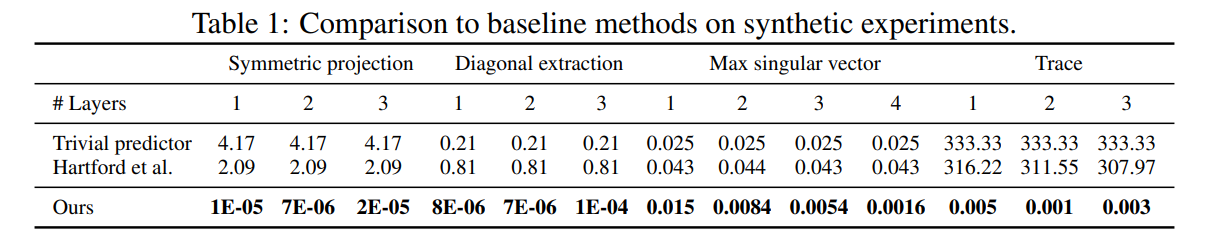
\includegraphics[width=0.98\textwidth]{../figures/synth.png}
    \end{center}
\end{frame}
%%%%%%%%%%%%%%%%%%%%%%%%%%%%%%%%%%%%%%%%%%%%%%%%%%%%%%%%%%%%%%%%%%%%%%%%%%%%%%
\begin{frame}{Expressive Power of Equivariant Networks}
    \begin{itemize}
        \item In previous lectures, we saw that a popular way to measure the expressivity of a GNN is by looking at the Weisfeiler-Lehman (WL) test.
        \pause
        \item The $k$-WL tests are a family of graph isomorphism tests that can distinguish between increasingly many non-isomorphic graphs.
        \item We want to show that for some $k$, our $k$-order networks can distinguish between non-isomorphic graphs just as well as the $k$-WL test.
    \end{itemize}
\end{frame}
%%%%%%%%%%%%%%%%%%%%%%%%%%%%%%%%%%%%%%%%%%%%%%%%%%%%%%%%%%%%%%%%%%%%%%%%%%%%%%
\begin{frame}{Expressive Power of Equivariant Networks}
    \begin{itemize}
        \item In Maron et al. (2019), the authors show that the $k$-order equivariant network is able to distinguish between non-isomorphic graphs just as well as the $k$-WL test.
        \item The model proposed is much more efficient than $k$-GNNs which are also equivalent to the $k$-WL test.
    \end{itemize}
\end{frame}
%%%%%%%%%%%%%%%%%%%%%%%%%%%%%%%%%%%%%%%%%%%%%%%%%%%%%%%%%%%%%%%%%%%%%%%%%%%%%%
\begin{frame}{Expressive Power of Equivariant Networks}
    \begin{itemize}
        \item The proof that the $k$-order equivariant network is able to distinguish between non-isomorphic graphs just as well as the $k$-WL test is quite complex.
        \item \pause
        \item In general, we can "simulate" the $k-1$-(F)WL algorithm using a $k$-order equivariant network if we have a sufficient number of parameters.
        \item \pause
        \item The information required to run the $k-1$-(F)WL algorithm is encoded in the input to the network.
    \end{itemize}
\end{frame}
%%%%%%%%%%%%%%%%%%%%%%%%%%%%%%%%%%%%%%%%%%%%%%%%%%%%%%%%%%%%%%%%%%%%%%%%%%%%%%
% Thank You Slide
\begin{frame}[plain]
    \centering
    \Huge Thank You!
\end{frame}

\end{document}
